\subsection{Настройка запуска по расписанию}
%\marginnote{\Date{Пт.}{27}{Янв.}{2023}}[-40pt]
%\setlist[1]{itemsep=-1pt}

\begin{itemize}
	\item  Выполняем команду для запуска планировщика
	
		\commandbox*{crontab -e} 	
%	\begin{tcolorbox}
%		
%		\begin{lstlisting}[language=bash]
%crontab -e
%		\end{lstlisting}
%	\end{tcolorbox}
	
	\item В открывшемся редакторе в конец файла добавить строку
	
	\commandbox*{* * * * *   /home/administrator/Workshift_load/src/wsh_load.py $HOME/command.log  2>&1} 	

		
%	\begin{tcolorbox}
%		
%		\begin{lstlisting}[language=Python,basicstyle= \footnotesize]
%* * * * *   /home/administrator/Workshift_load/src/wsh_load.py $HOME/command.log  2>&1
%		\end{lstlisting}

%	\end{tcolorbox}
	Здесь мы указываем периодичность запуска, полный путь к исполняемому скрипту, путь до файла в который будут выводиться сообщения планировщика.\ldots\todo[fancyline]{Finish sentence}
	Сохранить файл. Теперь при таких настройках скрипт будет запускаться каждую минуту. Для работы нужно выставить нужный интервал запуска.	Он выставляется в первой секции строки:
	
	\begin{figure}[H]
		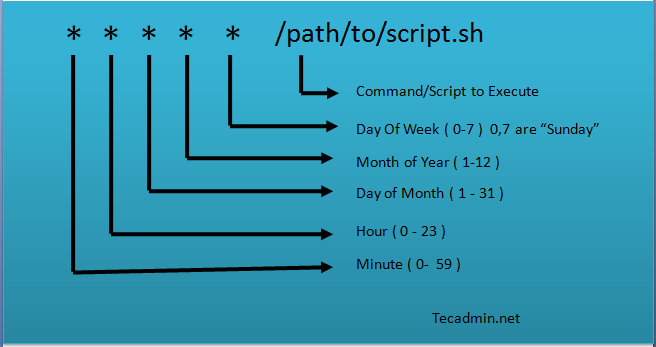
\includegraphics[width=0.95\textwidth]{crontab-2.png}
		\caption{<<Формат Linux Crontab>>.}
		\label{ris:crontab-2.png}
	\end{figure}
	
	\textcolor{RoyalBlue}{Синтаксис:
	*(Minute)*(Hour)*(Day of the Month)*(Month of the Year) *(Day of the Week) username <path to command/script to execute>}


	
	\begin{tabular}{|l|l|}
		
	\hline
	Минуты & Это значение может быть в пределах 0 — 59 \\
	\hline
Часы	& Это значение может быть в пределах 0 — 23 \\
	\hline
День месяца	& Это значение может быть в пределах 1 — 31 \\
	\hline
Месяц в году	& \vtop{\hbox{\strut Это значение поля находится в диапазоне от 1 до 12. }\hbox{\strut Так же можно использовать три первые буквы названия месяца, например: jan, feb, mar}}  \\
	\hline
День недели	& \vtop{\hbox{\strut Это значение поля находится в диапазоне от 0 до 7.}\hbox{\strut Где 0 и 7-воскресенье. 1-понедельник, 2-вторник и так далее}}  \\
	\hline
	\end{tabular}

\newpage	
	\textbf{Пример:}
	
	\textsl {Следующее выражение для выполнения задачи каждые 5 минут.}
	\begin{tcolorbox}
		
		\begin{lstlisting}[language=bash]
*/5 * * * * /home/administrator/Workshift_load/src/wsh_load.py
		\end{lstlisting}
	\end{tcolorbox}
	
	
\end{itemize}
